\clearpage
\subsubsection{one-hot法}
\label{subsubsec:lab4-task1-one-hot}

\paragraph{实验过程与关键代码}

one-hot法从DDT或LAT中提取所有非零位置，组成可达点列表\texttt{points}。随后对每个可达输入输出对设置一个二进制选择变量$\lambda_{a,b}$，并要求所有选择变量之和为1。这样，每次求解都恰好选中一个可达点。

在\texttt{one\_hot.py}中，通过\texttt{bits(a,b)}计算可达点的八位编码，并建立8个原始变量和相应的选择变量：
\begin{lstlisting}
V = [(a, b) for a in range(SIZE) for b in range(SIZE) if table[a][b] != 0]
x = model.addVars(8, vtype=gp.GRB.BINARY)
lam = model.addVars(V, vtype=gp.GRB.BINARY)
model.addConstr(lam.sum() == 1)
\end{lstlisting}

选择变量确定可达点后，还需要使$x$的每一位等于该点的对应坐标。对于第$j$位，只累加该位为1的可达点所对应的选择变量：
\begin{lstlisting}
for j in range(8):
    model.addConstr(x[j] == gp.quicksum(lam[p] for p in V if bits(*p)[j] == 1))
\end{lstlisting}

因此，模型包含1条选点等式和8条坐标恢复等式，共9条等式。由于可达点列表中的每个输入输出对互不相同，一组八位坐标也唯一确定被选中的$\lambda$。建立约束后，使用前面的解池参数分别枚举DDT模型与LAT模型。

\paragraph{实验结果与分析}

代码运行结果如图~\ref{fig:lab4-task1-one-hot}所示。
\begin{figure}[H]
    \centering
    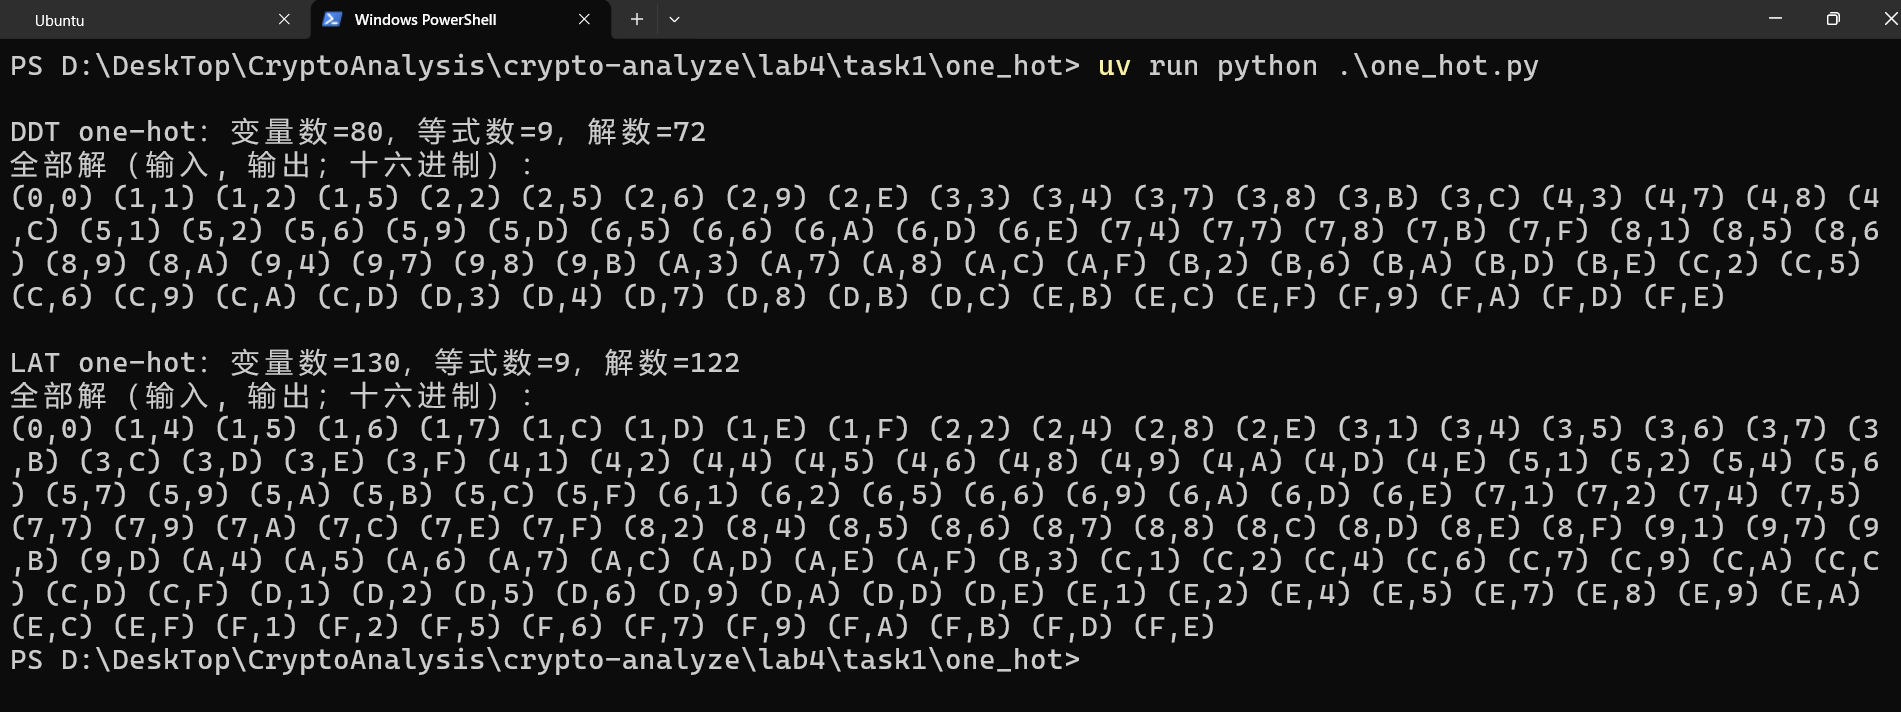
\includegraphics[width=\textwidth]{figures/task1/Grubi_solve1.png}
    \caption{one-hot法的DDT、LAT模型全解枚举结果}
    \label{fig:lab4-task1-one-hot}
\end{figure}

DDT模型有72个选择变量，加上8个原始变量，共$72+8=80$个二进制变量；

LAT模型对应$122+8=130$个二进制变量。两者均有9条等式，与上述建模过程一致。求解得到的DDT解数为72，LAT解数为122，按输入分组后与图~\ref{fig:lab4-task1-ddt-lat}中的非零项一致，所以说，one-hot法的建模与求解结果正确

图~\ref{fig:lab4-task1-one-hot-log}是开启Gurobi过程日志时的一次运行；当前脚本默认关闭过程日志，只打印最终枚举结果。
\begin{figure}[H]
    \centering
    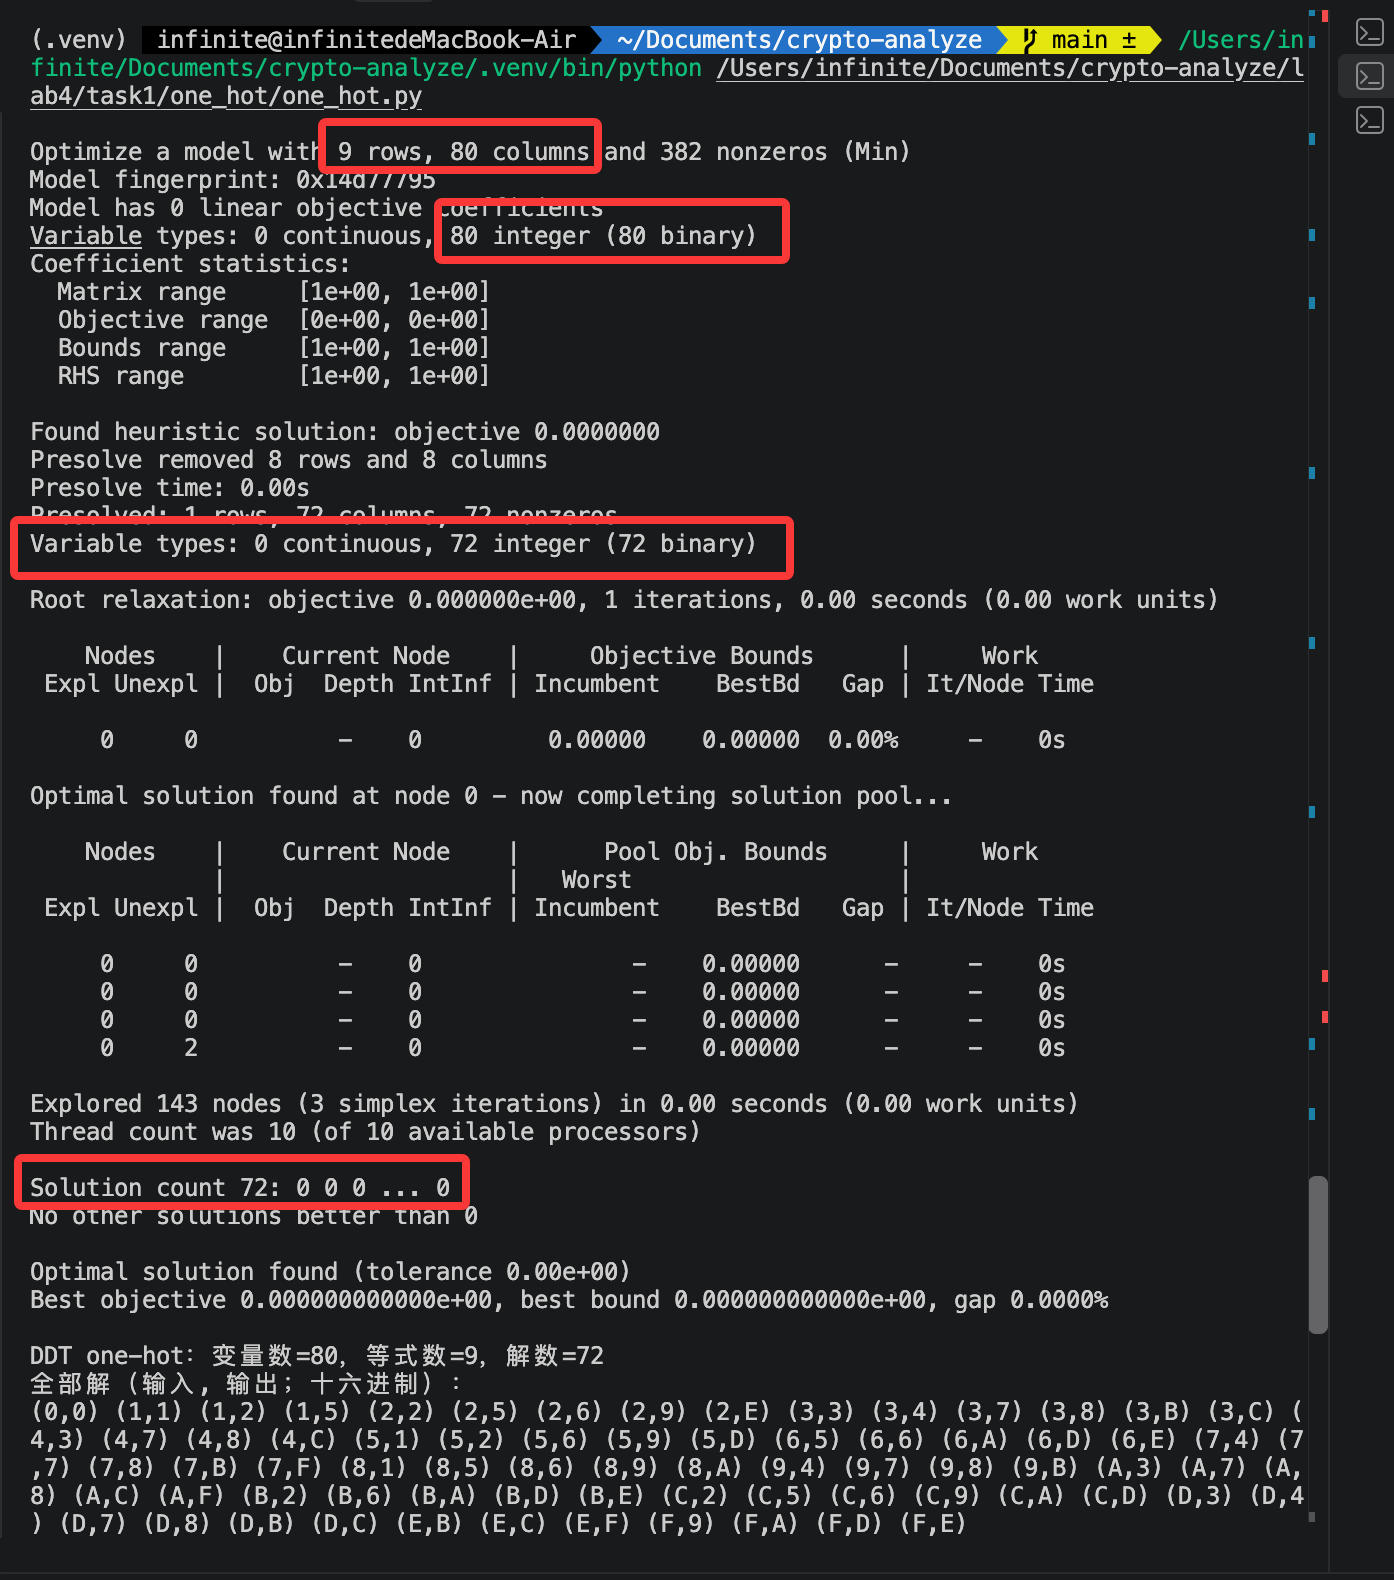
\includegraphics[width=\textwidth]{figures/one_hot.png}
    \caption{开启过程日志时的one-hot模型预求解信息}
    \label{fig:lab4-task1-one-hot-log}
\end{figure}

我们发现gurobi会进行一个presolve的流程，这会使得变量缩减到72个,因为剩下那8个变量其实就是我们的bits(a,b)

那这些是可以由$\lambda$计算出来的，所以就不需要保留，不过这个属于求解器内部的事了，我们还是按80个变量来算
